\chapter{$\PN[3]$ advection matrices}\label{app:C}
\comment{
Recall from \sref{sec:pn_op} that the steady-state $\PN$ system can be written in the operator form as follows (eq.
\eqref{eq:pn_op}):
\begin{equation}\label{eq:PN_ss_app}
	\PihPN (A+\Sigma_t-K) \PiPN\Phi = \PihPN q,
\end{equation}
where (in the monoenergetic case) 
$$
\begin{gathered}
A\psi(\br,\bomega) = \bomega\cdot\nabla\psi(\br,\bomega),\quad
\Sigma_t\psi(\br,\bomega) = \sigma_t(\br)\psi(\br,\bomega)\\
K\psi(\br,\bomega) = \intA[']{\kappa(\br,\bomega\cdot\bomega')\psi(\br,\bomega')}.
\end{gathered}         
$$
and for $\mat{F} = \col \{f_k\}_{\idxset{K}}$,
\begin{equation}\label{eq:pn_op_def_app}
\bigl(\PiPN\mat{F}\bigr)(\bomega) := \sum_{k=1}^{ K} f_k\Y{k}{}(\bomega), \quad
\PihPN f(\bomega) = \col \left\{(f, \Y{k}{})_{\Lp[2](\Sphere)}\right\}_{\idxset{K}}
\end{equation}
}
In this appendix, we investigate the advection matrices $\mat{A}_{P_N}^s$ ($s = x,y,z$) for the special case $N = 3$ 
(the statements that follow have been computationally verified to hold for $N = 1,2,\ldots,11$ using the symbolic 
system Mathematica 9.0).
It is more convenient for this analysis to consider the steady-state $\PN$ equations \eqref{eq:PN_ss_app} as a limit
of the time-dependent equations
\begin{equation}\label{eq:PN_ss_app}
	\PihPN \left(\pd{}{t} + A + \Sigma_t - K\right) \PiPN\Phi = \PihPN q,
\end{equation}
in which $\pd{\psi}{t} \to 0$, for time-independent boundary conditions and sources
\linebreak[4]\mbox{$q(\cdot,\cdot,t) = \text{const}$}.
Then, the advection matrices describe advection of neutrons introduced into the system by the boundary and internal
sources, which is in the steady-state limit perfectly balanced by their attenuation due to net effect of collisions of
all types.

$$
\scriptsize
\hspace*{-2cm}
\begin{aligned}
\mat{A}_{P_N}^x &=
\left[
\begin{array}{cccccccccccccccc}
 0 & 0 & 0 & \frac{1}{\sqrt{3}} & 0 & 0 & 0 & 0 & 0 & 0 & 0 & 0 & 0 & 0 & 0 & 0 \\
 0 & 0 & 0 & 0 & \frac{1}{\sqrt{5}} & 0 & 0 & 0 & 0 & 0 & 0 & 0 & 0 & 0 & 0 & 0 \\
 0 & 0 & 0 & 0 & 0 & 0 & 0 & \frac{1}{\sqrt{5}} & 0 & 0 & 0 & 0 & 0 & 0 & 0 & 0 \\
 \frac{1}{\sqrt{3}} & 0 & 0 & 0 & 0 & 0 & -\frac{1}{\sqrt{15}} & 0 & \frac{1}{\sqrt{5}} & 0 & 0 & 0 & 0 & 0 & 0 & 0 \\
 0 & \frac{1}{\sqrt{5}} & 0 & 0 & 0 & 0 & 0 & 0 & 0 & \sqrt{\frac{3}{14}} & 0 & -\frac{1}{\sqrt{70}} & 0 & 0 & 0 & 0 \\
 0 & 0 & 0 & 0 & 0 & 0 & 0 & 0 & 0 & 0 & \frac{1}{\sqrt{7}} & 0 & 0 & 0 & 0 & 0 \\
 0 & 0 & 0 & -\frac{1}{\sqrt{15}} & 0 & 0 & 0 & 0 & 0 & 0 & 0 & 0 & 0 & \sqrt{\frac{6}{35}} & 0 & 0 \\
 0 & 0 & \frac{1}{\sqrt{5}} & 0 & 0 & 0 & 0 & 0 & 0 & 0 & 0 & 0 & -\sqrt{\frac{3}{35}} & 0 & \frac{1}{\sqrt{7}} & 0 \\
 0 & 0 & 0 & \frac{1}{\sqrt{5}} & 0 & 0 & 0 & 0 & 0 & 0 & 0 & 0 & 0 & -\frac{1}{\sqrt{70}} & 0 & \sqrt{\frac{3}{14}} \\
 0 & 0 & 0 & 0 & \sqrt{\frac{3}{14}} & 0 & 0 & 0 & 0 & 0 & 0 & 0 & 0 & 0 & 0 & 0 \\
 0 & 0 & 0 & 0 & 0 & \frac{1}{\sqrt{7}} & 0 & 0 & 0 & 0 & 0 & 0 & 0 & 0 & 0 & 0 \\
 0 & 0 & 0 & 0 & -\frac{1}{\sqrt{70}} & 0 & 0 & 0 & 0 & 0 & 0 & 0 & 0 & 0 & 0 & 0 \\
 0 & 0 & 0 & 0 & 0 & 0 & 0 & -\sqrt{\frac{3}{35}} & 0 & 0 & 0 & 0 & 0 & 0 & 0 & 0 \\
 0 & 0 & 0 & 0 & 0 & 0 & \sqrt{\frac{6}{35}} & 0 & -\frac{1}{\sqrt{70}} & 0 & 0 & 0 & 0 & 0 & 0 & 0 \\
 0 & 0 & 0 & 0 & 0 & 0 & 0 & \frac{1}{\sqrt{7}} & 0 & 0 & 0 & 0 & 0 & 0 & 0 & 0 \\
 0 & 0 & 0 & 0 & 0 & 0 & 0 & 0 & \sqrt{\frac{3}{14}} & 0 & 0 & 0 & 0 & 0 & 0 & 0 \\
\end{array}
\right]\\[5em]
\mat{A}_{P_N}^y &=
\left[
\begin{array}{cccccccccccccccc}
 0 & \frac{1}{\sqrt{3}} & 0 & 0 & 0 & 0 & 0 & 0 & 0 & 0 & 0 & 0 & 0 & 0 & 0 & 0 \\
 \frac{1}{\sqrt{3}} & 0 & 0 & 0 & 0 & 0 & -\frac{1}{\sqrt{15}} & 0 & -\frac{1}{\sqrt{5}} & 0 & 0 & 0 & 0 & 0 & 0 & 0 \\
 0 & 0 & 0 & 0 & 0 & \frac{1}{\sqrt{5}} & 0 & 0 & 0 & 0 & 0 & 0 & 0 & 0 & 0 & 0 \\
 0 & 0 & 0 & 0 & \frac{1}{\sqrt{5}} & 0 & 0 & 0 & 0 & 0 & 0 & 0 & 0 & 0 & 0 & 0 \\
 0 & 0 & 0 & \frac{1}{\sqrt{5}} & 0 & 0 & 0 & 0 & 0 & 0 & 0 & 0 & 0 & -\frac{1}{\sqrt{70}} & 0 & -\sqrt{\frac{3}{14}} \\
 0 & 0 & \frac{1}{\sqrt{5}} & 0 & 0 & 0 & 0 & 0 & 0 & 0 & 0 & 0 & -\sqrt{\frac{3}{35}} & 0 & -\frac{1}{\sqrt{7}} & 0 \\
 0 & -\frac{1}{\sqrt{15}} & 0 & 0 & 0 & 0 & 0 & 0 & 0 & 0 & 0 & \sqrt{\frac{6}{35}} & 0 & 0 & 0 & 0 \\
 0 & 0 & 0 & 0 & 0 & 0 & 0 & 0 & 0 & 0 & \frac{1}{\sqrt{7}} & 0 & 0 & 0 & 0 & 0 \\
 0 & -\frac{1}{\sqrt{5}} & 0 & 0 & 0 & 0 & 0 & 0 & 0 & \sqrt{\frac{3}{14}} & 0 & \frac{1}{\sqrt{70}} & 0 & 0 & 0 & 0 \\
 0 & 0 & 0 & 0 & 0 & 0 & 0 & 0 & \sqrt{\frac{3}{14}} & 0 & 0 & 0 & 0 & 0 & 0 & 0 \\
 0 & 0 & 0 & 0 & 0 & 0 & 0 & \frac{1}{\sqrt{7}} & 0 & 0 & 0 & 0 & 0 & 0 & 0 & 0 \\
 0 & 0 & 0 & 0 & 0 & 0 & \sqrt{\frac{6}{35}} & 0 & \frac{1}{\sqrt{70}} & 0 & 0 & 0 & 0 & 0 & 0 & 0 \\
 0 & 0 & 0 & 0 & 0 & -\sqrt{\frac{3}{35}} & 0 & 0 & 0 & 0 & 0 & 0 & 0 & 0 & 0 & 0 \\
 0 & 0 & 0 & 0 & -\frac{1}{\sqrt{70}} & 0 & 0 & 0 & 0 & 0 & 0 & 0 & 0 & 0 & 0 & 0 \\
 0 & 0 & 0 & 0 & 0 & -\frac{1}{\sqrt{7}} & 0 & 0 & 0 & 0 & 0 & 0 & 0 & 0 & 0 & 0 \\
 0 & 0 & 0 & 0 & -\sqrt{\frac{3}{14}} & 0 & 0 & 0 & 0 & 0 & 0 & 0 & 0 & 0 & 0 & 0 \\
\end{array}
\right]
\end{aligned}
$$
\newpage
$$
\scriptsize
\hspace*{-2cm}
\mat{A}_{P_N}^z =
\left[
\begin{array}{cccccccccccccccc}
 0 & 0 & \frac{1}{\sqrt{3}} & 0 & 0 & 0 & 0 & 0 & 0 & 0 & 0 & 0 & 0 & 0 & 0 & 0 \\
 0 & 0 & 0 & 0 & 0 & \frac{1}{\sqrt{5}} & 0 & 0 & 0 & 0 & 0 & 0 & 0 & 0 & 0 & 0 \\
 \frac{1}{\sqrt{3}} & 0 & 0 & 0 & 0 & 0 & \frac{2}{\sqrt{15}} & 0 & 0 & 0 & 0 & 0 & 0 & 0 & 0 & 0 \\
 0 & 0 & 0 & 0 & 0 & 0 & 0 & \frac{1}{\sqrt{5}} & 0 & 0 & 0 & 0 & 0 & 0 & 0 & 0 \\
 0 & 0 & 0 & 0 & 0 & 0 & 0 & 0 & 0 & 0 & \frac{1}{\sqrt{7}} & 0 & 0 & 0 & 0 & 0 \\
 0 & \frac{1}{\sqrt{5}} & 0 & 0 & 0 & 0 & 0 & 0 & 0 & 0 & 0 & 2 \sqrt{\frac{2}{35}} & 0 & 0 & 0 & 0 \\
 0 & 0 & \frac{2}{\sqrt{15}} & 0 & 0 & 0 & 0 & 0 & 0 & 0 & 0 & 0 & \frac{3}{\sqrt{35}} & 0 & 0 & 0 \\
 0 & 0 & 0 & \frac{1}{\sqrt{5}} & 0 & 0 & 0 & 0 & 0 & 0 & 0 & 0 & 0 & 2 \sqrt{\frac{2}{35}} & 0 & 0 \\
 0 & 0 & 0 & 0 & 0 & 0 & 0 & 0 & 0 & 0 & 0 & 0 & 0 & 0 & \frac{1}{\sqrt{7}} & 0 \\
 0 & 0 & 0 & 0 & 0 & 0 & 0 & 0 & 0 & 0 & 0 & 0 & 0 & 0 & 0 & 0 \\
 0 & 0 & 0 & 0 & \frac{1}{\sqrt{7}} & 0 & 0 & 0 & 0 & 0 & 0 & 0 & 0 & 0 & 0 & 0 \\
 0 & 0 & 0 & 0 & 0 & 2 \sqrt{\frac{2}{35}} & 0 & 0 & 0 & 0 & 0 & 0 & 0 & 0 & 0 & 0 \\
 0 & 0 & 0 & 0 & 0 & 0 & \frac{3}{\sqrt{35}} & 0 & 0 & 0 & 0 & 0 & 0 & 0 & 0 & 0 \\
 0 & 0 & 0 & 0 & 0 & 0 & 0 & 2 \sqrt{\frac{2}{35}} & 0 & 0 & 0 & 0 & 0 & 0 & 0 & 0 \\
 0 & 0 & 0 & 0 & 0 & 0 & 0 & 0 & \frac{1}{\sqrt{7}} & 0 & 0 & 0 & 0 & 0 & 0 & 0 \\
 0 & 0 & 0 & 0 & 0 & 0 & 0 & 0 & 0 & 0 & 0 & 0 & 0 & 0 & 0 & 0 \\
\end{array}
\right]
$$

By computing the norms of matrices
$$
D_{xy} := \left(\mat{A}_{P_N}^x\right)^T \mat{A}_{P_N}^y - \left(\mat{A}_{P_N}^y\right)^T \mat{A}_{P_N}^x
$$
(similarly for the remaining combinations of $x$,$y$), i.e. (for the largest singular value norm)
$$
	\norm{D_{xy}} = \norm{D_{yz}} = \norm{D_{xz}} = \frac{2}{5}
$$
we observe that the matrices
$A_{P_3}^s$ ($s = x,y,z$) do not commute and hence can not be simultaneously 
diagonalized by a common eigenvector matrix. Consequently, the radiation advected by these matrices cannot be decomposed into plane-waves propagating in distinct directions (as in 
the case of the $\SN$ approximation), but rather consists of a combination of waves propagating in the infinitely many 
directions in $\R[3]$.

Let us now take an arbitrary fixed direction $\bn = [n_x,n_y,n_z]$ from this infinite set. 
The matrix
$$
	\mat{A}_{P_N}^{\bn} = n_x \mat{A}_{P_N}^x + n_y \mat{A}_{P_N}^y + n_z \mat{A}_{P_N}^z,
$$
displayed below for the case $N = 3$, shows that at most 7 unknowns are coupled in the $\PN[3]$ system, as the
capture matrix $C = \Sigma_t - K$ is diagonal (Corollary \label{cor:capture} on p.~\pageref{cor:capture}).

\begin{figure}[htb]
\hspace*{-1.1cm}
  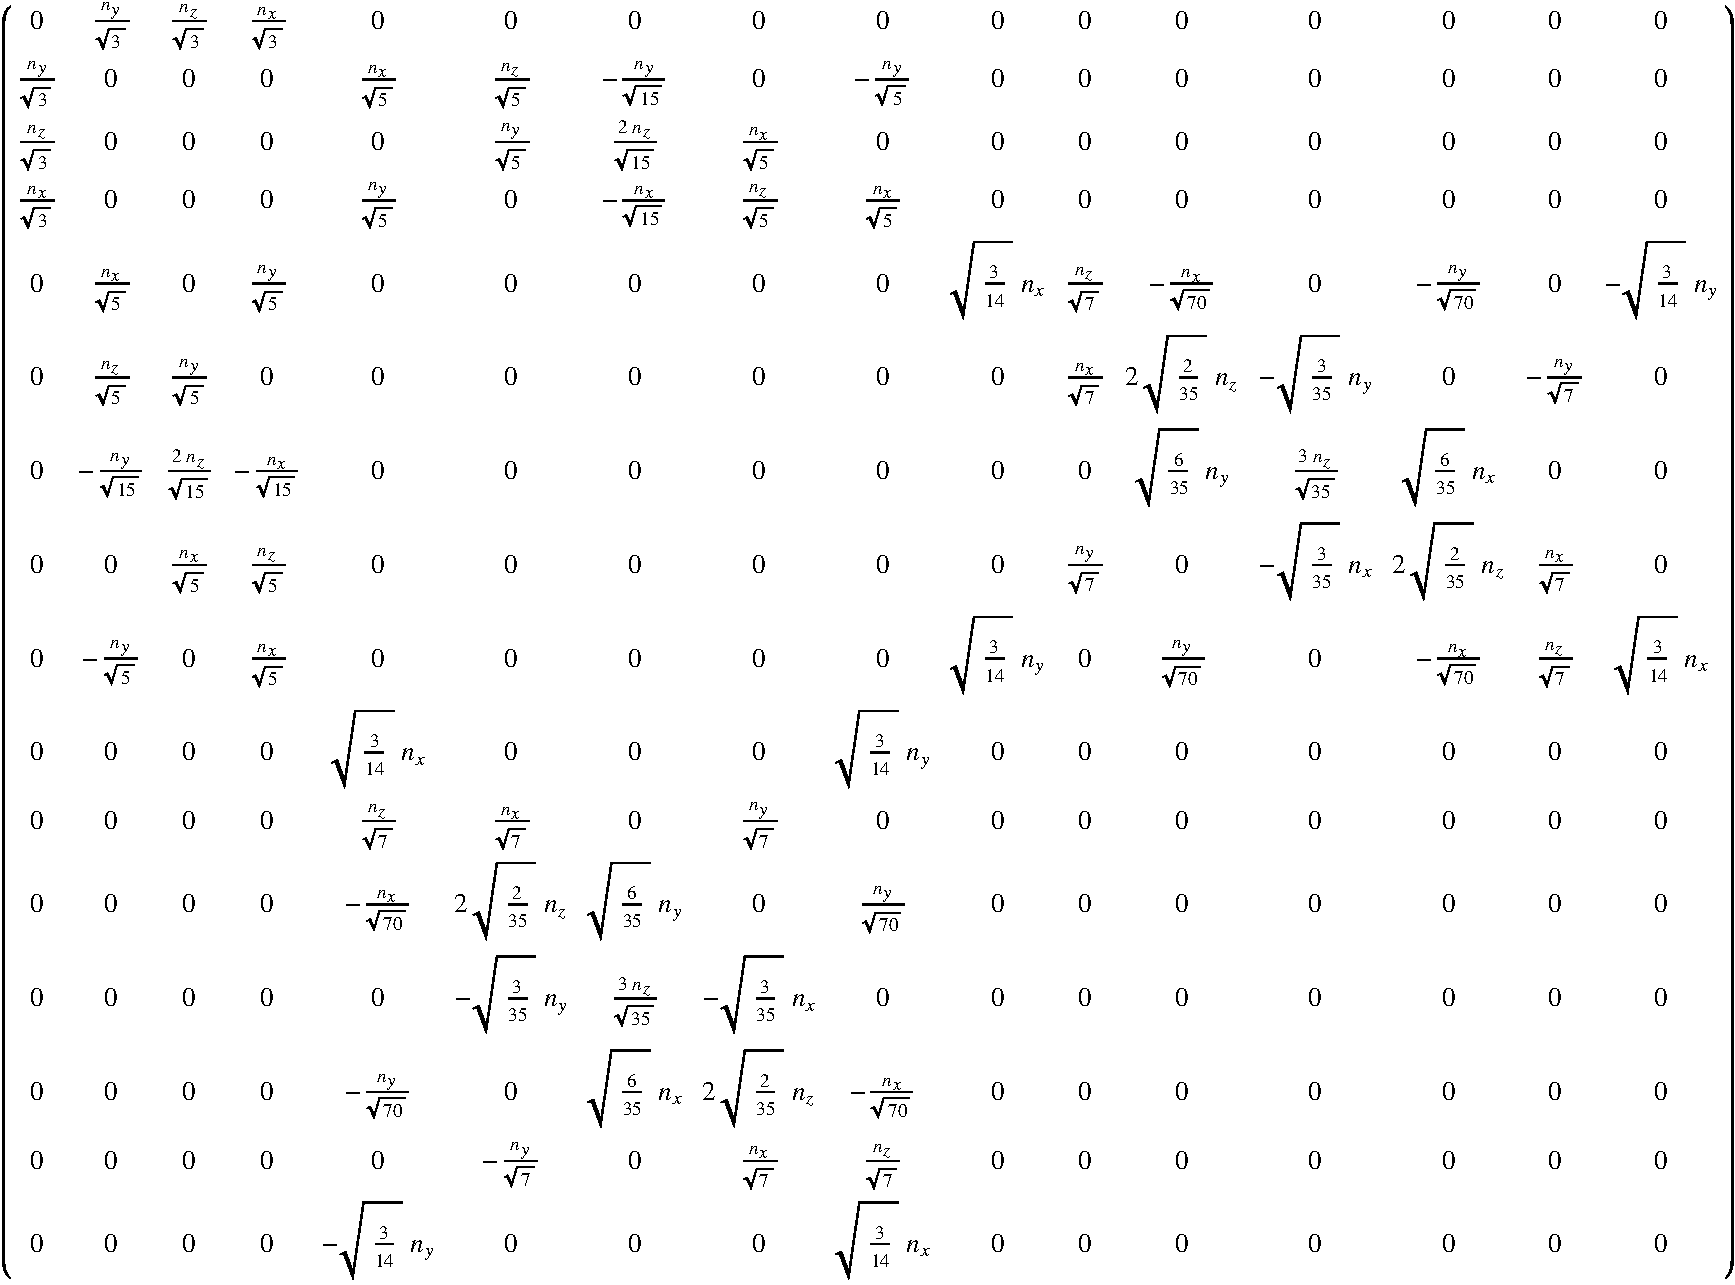
\includegraphics[scale=.575]{nA_P3}
  \caption{$\mat{A}_{\PN[3]}^{\bn}$}
  \label{fig:nAP3}
\end{figure}

Its eigendecomposition
shows that speed of propagation is uniform for all $\bn\in\R[3]$, given by the eigenvalues corresponding to the case
$\norm{\bn} = 1$ (written with their multiplicities):
$$
\begin{multlined}
\textstyle
\left\{0,0,0,0,-\sqrt{\frac{3}{7}},-\sqrt{\frac{3}{7}},\sqrt{\frac{3}{7}},\sqrt{\frac{3}{7}},-\frac{1}{\sqrt{7}},
-\frac{1}{\sqrt{7}},\frac{1}{\sqrt{7}},\frac{1}{\sqrt{7}},\right.\\
\textstyle
\left.-\sqrt{\frac{1}{35} \left(15-2 \sqrt{30}\right)},
\sqrt{\frac{1}{35} \left(15-2 \sqrt{30}\right)},-\sqrt{\frac{1}{35} \left(15+2 \sqrt{30}\right)},\sqrt{\frac{1}{35} 
\left(15+2 \sqrt{30}\right)}\right\}
\end{multlined} 
$$

\newpage
\begin{remark}[\textsc{Time dependent problems}] 
Let us compare the nullspaces of $\PN[2]$ advection matrix $\mat{A}_{P_2}^{\bn}$: 
$$
\left[
\begin{array}{ccc}
 \frac{\sqrt{\frac{3}{5}} \left(n_z^2-1\right)}{1-2 n_y^2} & \frac{2 \sqrt{\frac{3}{5}} n_x n_z}{1-2 n_y^2} & \frac{\frac{3 n_z^2}{2 n_y^2-1}+1}{\sqrt{5}} \\
 0 & 0 & 0 \\
 0 & 0 & 0 \\
 0 & 0 & 0 \\
 \frac{n_x \left(n_z^2-2 n_y^2\right)}{n_y \left(2 n_y^2-1\right)} & -\frac{n_z-2 n_z^3}{n_y-2 n_y^3} & \frac{\sqrt{3} n_x n_z^2}{n_y-2 n_y^3} \\
 -\frac{n_z-n_z^3}{n_y-2 n_y^3} & \frac{n_x \left(-2 n_y^2-2 n_z^2+1\right)}{n_y \left(2 n_y^2-1\right)} & \frac{\sqrt{3} n_z \left(2 n_y^2+n_z^2-1\right)}{n_y \left(2 n_y^2-1\right)} \\
 0 & 0 & 1 \\
 0 & 1 & 0 \\
 1 & 0 & 0 \\
\end{array}
\right]
$$

\noindent and $\PN[3]$ advection matrix $\mat{A}_{P_3}^{\bn}$:

$$
\hspace*{-3.5cm}
\scriptsize
\left[
\begin{array}{cccc}
 0 & 0 & 0 & 0 \\
 \frac{\sqrt{\frac{15}{14}} n_x \left(n_z^2-1\right)}{n_y \left(4 n_y^2-3\right)} & \frac{\sqrt{\frac{5}{7}} n_z \left(2 n_y^2+3 n_z^2-3\right)}{n_y \left(4 n_y^2-3\right)} & \frac{n_x \left(-4 n_y^2-15 n_z^2+3\right)}{\sqrt{14} n_y \left(4 n_y^2-3\right)} & \frac{\sqrt{\frac{3}{7}} n_z \left(-4 n_y^2-5 n_z^2+3\right)}{n_y \left(4 n_y^2-3\right)} \\
 -\frac{\sqrt{\frac{30}{7}} n_x n_z \left(n_z^2-1\right)}{8 n_y^4-10 n_y^2+3} & -\frac{\sqrt{\frac{5}{7}} \left(2 n_z^2-1\right) \left(4 n_y^2+3 n_z^2-3\right)}{8 n_y^4-10 n_y^2+3} & \frac{5 \sqrt{\frac{2}{7}} n_x \left(n_y^2-3 n_x^2\right) n_z}{8 n_y^4-10 n_y^2+3} & \frac{\sqrt{\frac{3}{7}} \left(8 n_y^4-10 n_y^2+10 n_z^4+5 \left(4 n_y^2-3\right) n_z^2+3\right)}{8 n_y^4-10 n_y^2+3} \\
 -\frac{\sqrt{\frac{15}{14}} \left(2 n_y^2-2 n_z^2-1\right) \left(n_z^2-1\right)}{8 n_y^4-10 n_y^2+3} & \frac{2 \sqrt{\frac{5}{7}} n_x n_z \left(2 n_y^2-3 n_z^2\right)}{8 n_y^4-10 n_y^2+3} & \frac{8 n_y^4-10 \left(n_z^2+1\right) n_y^2-30 n_z^4+15 n_z^2+3}{\sqrt{14} \left(8 n_y^4-10 n_y^2+3\right)} & \frac{10 \sqrt{\frac{3}{7}} n_x n_z^3}{8 n_y^4-10 n_y^2+3} \\
 0 & 0 & 0 & 0 \\
 0 & 0 & 0 & 0 \\
 0 & 0 & 0 & 0 \\
 0 & 0 & 0 & 0 \\
 0 & 0 & 0 & 0 \\
 \frac{n_x \left(-8 n_y^4+\left(4 n_z^2+6\right) n_y^2-3 n_z^4+n_z^2-1\right)}{n_y \left(8 n_y^4-10 n_y^2+3\right)} & \frac{\sqrt{\frac{3}{2}} n_z \left(-6 n_z^4+5 n_z^2-1\right)}{n_y \left(8 n_y^4-10 n_y^2+3\right)} & \frac{\sqrt{15} n_x n_z^2 \left(3 n_z^2-1\right)}{n_y \left(8 n_y^4-10 n_y^2+3\right)} & \frac{\sqrt{\frac{5}{2}} n_z^3 \left(4 n_y^2+6 n_z^2-5\right)}{n_y \left(8 n_y^4-10 n_y^2+3\right)} \\
 \frac{\sqrt{\frac{3}{2}} n_z \left(-4 n_z^4+5 n_z^2-1\right)}{n_y \left(8 n_y^4-10 n_y^2+3\right)} & -\frac{n_x \left(2 n_y^2-3 n_z^2\right) \left(4 n_y^2+4 n_z^2-3\right)}{n_y \left(8 n_y^4-10 n_y^2+3\right)} & \frac{\sqrt{\frac{5}{2}} n_z \left(4 n_y^2+3 n_z^2-3\right) \left(4 n_z^2-1\right)}{n_y \left(8 n_y^4-10 n_y^2+3\right)} & \frac{\sqrt{15} n_x n_z^2 \left(-4 n_y^2-4 n_z^2+3\right)}{n_y \left(8 n_y^4-10 n_y^2+3\right)} \\
 \frac{\sqrt{15} n_x n_z^2 \left(n_z^2-1\right)}{n_y \left(8 n_y^4-10 n_y^2+3\right)} & \frac{\sqrt{\frac{5}{2}} n_z \left(2 n_z^2-1\right) \left(4 n_y^2+3 n_z^2-3\right)}{n_y \left(8 n_y^4-10 n_y^2+3\right)} & -\frac{n_x \left(8 n_y^4-10 n_y^2+15 n_z^4+5 \left(4 n_y^2-3\right) n_z^2+3\right)}{n_y \left(8 n_y^4-10 n_y^2+3\right)} & -\frac{\sqrt{\frac{3}{2}} n_z \left(16 n_y^4+20 \left(n_z^2-1\right) n_y^2+10 n_z^4-15 n_z^2+6\right)}{n_y \left(8 n_y^4-10 n_y^2+3\right)} \\
 0 & 0 & 0 & 1 \\
 0 & 0 & 1 & 0 \\
 0 & 1 & 0 & 0 \\
 1 & 0 & 0 & 0 \\
\end{array}
\right]
$$

\noindent Unlike the $\PN[3]$ approximation, we can see that the $\PN[2]$ approximation contains in its advection
nullspace nonzero components of the 0-th moment of angular flux, which is proportional to the scalar flux (total spatial neutron 
density). Therefore, as a consequence of $\PN[2]$ approximation, not all scalar flux components are propagated by the
action $\mat{A}_{P_2}^{\bn} \Psi$. It turns out that this is true for any even-order $\PN$ approximation, which is
``probably the most salient argument why even-order expansions should be shunned for time dependent problems'' 
\cite[p. 20]{McClarren5}.
\end{remark}
  